\documentclass[../main.tex]{subfiles}
\begin{document}
\chapter{Laplace's and Poisson's Equations}
\section{Poisson's Equation and Boundary Conditions}
\begin{remark}[Recap]
  Recall from \cref{secLaplacian} that $\nabla^2 \phi$ is just the divergence of $\nabla \phi$, that is:
  \[
    \nabla^2 \phi = \nabla \cdot (\nabla \phi) = \pderiv[2]{\phi}{x} + \pderiv[2]{\phi}{y} + \pderiv[2]{\phi}{z}
  \]
\end{remark}
\subsection{Definitions}
\begin{definition}[Poisson's Equation]
  \textit{Poisson's equation} is:
  \label{poissonsEquation}
  \[
    \nabla^2 \phi = f,\ \vec{x} \in \mathscr{D}
  \]
  where $\phi(\vec{x})$ is an unknown scalar field, $f(\vec{x})$ is the specified \textit{source term} and $\mathscr{D}$ is some domain in which we would like to solve the equation in.
\end{definition}
\begin{definition}[Laplace's Equation]
  \textit{Laplace's equation} is a special case of Poisson's equation with $f = 0$, that is:
  \label{laplacesEquation}
  \[
    \nabla^2 \phi = 0,\ \vec{x} \in \mathscr{D}
  \]
\end{definition}
We also need boundary conditions on $\partial \mathscr{D}$.
Usually, they are either \textit{Dirichlet} or \textit{von Neumann} boundary conditions.

Dirichlet boundary conditions specific what the function is equal to on the boundary.
\begin{definition}[Dirichlet Boundary Conditions]
  \textit{Dirichlet boundary conditions} are boundary conditions of the form:
  \[
    \phi = g,\ \vec{x} \in \partial \mathscr{D}
  \]
\end{definition}
Whereas, von Neumann boundary conditions specify what normal derivative, i.e. the directional derivative (\cref{directionalDerivative}) along the normal, is at the boundary.
\begin{definition}[Von Neumman Boundary Conditions]
  \textit{Von Neumann boundary conditions} are of the form:
  \[
    \pderiv{\phi}{\vec{n}} = g,\ \vec{x} \in \partial\mathscr{D}
  \]
  where $\vec{g}(\vec{x})$ is a function specified on the boundary $\partial \mathscr{D}$.
\end{definition}
\begin{remark}[Notation]
  Recall from \cref{greensIdentities} that we defined the notation:
  \[
    \pderiv{\phi}{\vec{n}} \equiv \vec{n} \cdot \nabla \phi
  \]
\end{remark}
\subsection{Examples}
These equations typically arise in problems that can be expressed in terms of potentials.
\begin{example}[Electrostatics]
  In electrostatics, we use Maxwell's equations but restrict everything to be independent of time.
  Since $\vec{B}$ is constant in time, from \cref{maxwell3}, we see that $\nabla \times \vec{E} = \vec{0}$.
  This means that $\vec{E}$ is irrotational and so, in simply connected domain, it can be expressed in terms of an electric potential $\phi(\vec{x})$:
  \[
    \vec{E} = - \nabla \phi
  \]
  where the minus sign is included by convention.

  Then, using $\nabla \cdot \vec{E} = \frac{\rho}{\varepsilon_0}$ (\cref{maxwell1}), we obtain:
  \begin{equation}
    \nabla^2 \phi = - \frac{\rho}{\varepsilon_0} \label{laplaceElectrostatic}
  \end{equation}
  where $\rho(\vec{x})$ is the charge density.
  This is Poisson's equation (\cref{poissonsEquation}) with source term $f(\vec{x}) = -\frac{\rho}{\varepsilon_0}$.
\end{example}
\begin{example}[Examples of Solving Poisson's and Laplace's Equations]
  \begin{enumerate}
    \item Solve Laplace's equation (\cref{laplacesEquation}) in the square domain $0 \leq x, y \leq 1$ in $\R^2$ subject to the Dirichlet boundary condition:
      \begin{align*}
        \phi(x, 0) = 0,\ \phi(x, 1) = 0,\ \phi(0, y) = 0,\ \phi(1, y) = \sin(\pi y)
      \end{align*}
      Note that this is a valid Dirichlet boundary condition as $\phi$ is defined over the entire boundary.

      For now, we will guess a separable solution of the form $\phi(x, y) = p(x)q(y)$.
      Applying the boundary condition on $\phi(1, y)$, we see that $q(y) = A \sin \pi y$ where $A = \frac{1}{p(1)}$.

      If we then substitute this back into Laplace's equation, we have:
      \[
        0 = \nabla^2 \phi = \pderiv[2]{\phi}{x} + \pderiv[2]{\phi}{y} = p''(x)q(y) + p(x)q''(y) = A(p'' - \pi^2 p)\sin(\pi y)
      \]
      Since this has to be true for all $\vec{x}$ in the domain, we must have $p'' - \pi^2p = 0\ \forall x$ and so $p(x) = B \sinh \pi x + C \cosh \pi x$.
      Finally, we can match the other boundary conditions by taking $B = 1$ and $C = 0$ so a solution to the equation is:
      \[
        \phi(x, y) = \frac{\sinh \pi x \sin \pi y}{\sinh \pi}
      \]
      We will show later that this solution must be unique and so this is \textbf{the} solution.
    \item Solve Poisson's equation $\nabla^2 \phi = r$ in the domain $r < 1$  in $\R^3$ with the Dirichlet boundary condition $\phi = 0$ on $r = 1$.

      Because of the spherical symmetry, it is a good idea to look for a solution of the form $\phi = \phi(r)$ only.

      Recall from \cref{laplacianSphericalSymmetry} that for a radially symmetric scalar field $\phi(r)$, we have:
      \[
        \nabla^2 \phi = \phi''(r) + \frac{2\phi'(r)}{r} = \frac{1}{r^2}\deriv{}{r}(r^2 \phi'(r)) = \frac{1}{r}\deriv[2]{}{r}(r\phi(r))
      \]
      Using the final expression, we have:
      \begin{align*}
        &\frac{1}{r}(r \phi)'' = r \\
        \implies& r \phi = \frac{1}{12}r^4 + Ar + B \\
        \implies& \phi = \frac{1}{12}r^3 + A + \frac{B}{r}
      \end{align*}
      Firstly, we must have $B = 0$, otherwise $\phi$ is undefined at $r = 0$ which is in the domain.
      On the boundary $r = 1$ and $\phi = 0$ so $A = -\frac{1}{12}$.
      Therefore the solution is:
      \[
        \phi = \frac{1}{12}(r^3 - 1)
      \]
    \item Solve Laplace's equation in $1 < r < 2$ in $\R^3$ with mixed boundary conditions $\phi = 0$ on $r = 1$ (Dirichlet) and $\pderiv{\phi}{\vec{n}} = 1$ on $r = 2$ (von Neumann).

      Again, due to the radial symmetry, we try $\phi = \phi(r)$.
      Again applying the identity for $\nabla^2 \phi$, we have:
      \[
        \frac{1}{r}(r \phi)'' = 0 \implies \phi = A + \frac{B}{r}
      \]
      Note that $r = 0$ is not problematic here because we are working with $1 < r < 2$ so $B$ does not have to be 0.
      Applying the Dirichlet boundary condition, on $r = 1$, $\phi = 0$ and so $A + B = 0$.
      Applying the von Neumann boundary condition, on $r = 2$ the normal is $\vec{n} = \vec{e}_r$ so $\pderiv{\phi}{\vec{n}} = \vec{e}_r \cdot \nabla \phi$.
      This is just the radial component of $\nabla \phi$ which is $\pderiv{\phi}{r}$ and so the boundary condition requires that $\at{\pderiv{\phi}{r}}{r = 2} = 1$.
      Thus $-\frac{1}{4}B = 1$ and so the solution is:
      \[
        \phi(r) = 4\left(1 - \frac{1}{r}\right)
      \]
  \end{enumerate}
\end{example}
\begin{remark}[Advice]
  You should be on the lookout for when your general solution has points at which it is undefined in the domain.
  In these case case you need to set the arbitrary constants appropriately to remove this issue.
  Often exam questions will require you to do this otherwise you will be left with an undetermined constant.
\end{remark}
\subsection{Superposition of Solutions}
The Laplacian operator $\nabla^2$ is \textit{linear}, that is:
\[
  \nabla^2(\alpha \phi_1 + \beta \phi_2) = \alpha \nabla^2 \phi_1 + \beta \nabla^2 \phi_2
\]
for any constants $\alpha$ and $\beta$.
This means we can solve $\nabla^2 \phi = f_1 + f_2$ in $\mathscr{D}$ using the \textit{superposition} $\phi = \phi_1 + \phi_2$ where $\nabla^2 \phi_1 = f_1$ and $\nabla^2 \phi_2 = f_2$.

To solve Poisson's equation with Dirichlet boundary conditions:
\[
  \nabla^2 \phi = f \text{ in } \mathscr{D},\ \phi = g \text{ on } \partial \mathscr{D}
\]
it is sometimes useful to split the problem into two separate problems:
\begin{align*}
  \nabla^2 \phi_1 = f \text{ in } \mathscr{D} \text{ and } \phi_1 = 0 \text{ on } \partial \mathscr{D} \\
  \nabla^2 \phi_2 = 0 \text{ in } \mathscr{D} \text{ and } \phi_2 = g \text{ on } \partial \mathscr{D}
\end{align*}
We can then solve each problem separately so that $\phi = \phi_1 + \phi_2$ satisfies the original problem.
\subsection{Consistency for von Neumann Boundary Conditions}
\nonexaminable
Consider the problem with von Neumann boundary conditions:
\[
  \nabla^2 \phi = f \text{ in } \mathscr{D} \text{ and } \pderiv{\phi}{\vec{n}} = g \text{ on } \mathscr{D}
\]
If such as solution exists, then we have:
\begin{align*}
  \int_{\mathscr{D}} f \d{V} &= \int_{\mathscr{D}} \nabla \cdot (\nabla \phi) \d{V} \\
                             &= \int_{\partial \mathscr{D}} \nabla \phi \cdot \d{\vec{S}} \text{ by divergence theorem (\cref{divergenceTheorem})}\\
                             &= \int_{\partial S} g \d{S} \text{ using the boundary condition}
\end{align*}
Therefore, if $\int_{\mathscr{D}} f \d{V} \neq \int_{\partial \mathscr{D}} g \d{S}$, the problem is ill-posed and so there is no solution for $\phi$.
This means for von Neumann boundary conditions, we cannot just specify any function $g$ whereas for Dirichlet boundary conditions, there are no such constraints.
\section{Uniqueness of Solutions}
\label{uniquenessOfSolutions}
\begin{theorem}[Uniqueness with Dirichlet Boundary Conditions]
  The solution to Poisson's (or Laplace's) equation with Dirichlet boundary conditions is unique.
\end{theorem}
\begin{remark}[Exams]
  This proof is examined regularly in Tripos papers.
\end{remark}
\begin{proof}
  Suppose that $\phi_1$ and $\phi_2$ are both solutions to the problem:
  \[
    \nabla^2 \phi = f \text{ in } \mathscr{D} \text{ and } \phi = g \text{ on } \partial \mathscr{D}
  \]
  Define $\psi = \phi_1 - \phi_2$.
  We would like to show that $\psi$ is identically 0.

  By linearity of $\nabla^2$, $\psi$ is a solution to the problem:
  \[
    \nabla^2 \psi = 0 \text{ in } \mathscr{D} \text{ and } \psi = 0 \text{ on } \partial \mathscr{D}
  \]
  We can then apply the divergence theorem to $\vec{F} = \psi \nabla \psi$.
  Since $\psi = 0$ on $\partial \mathscr{D}$, we have:
  \[
    \int_{\mathscr{D}} \nabla \cdot (\psi \nabla \psi) \d{V} = \int_{\partial \mathscr{D}} \psi \nabla \psi \cdot \d{\vec{S}} = 0
  \]
  We can rewrite the left hand side of this using an identity from \cref{vectorIdentities}:
  \begin{align*}
    \int_{\mathscr{D}} \nabla \cdot (\psi \nabla \psi) \d{x} = \int_{\mathscr{D}} (\nabla \psi \cdot \nabla \psi + \cancelto{0}{\psi \nabla^2 \psi}) \d{V} = \int_{\mathscr{D}} |\nabla \psi|^2 \d{V}
  \end{align*}
  Thus $\int_{\mathscr{D}} |\nabla \psi|^2 \d{V} = 0$.
  Since $|\nabla \psi|^2 \geq 0$, we must have $|\nabla \psi| = 0 \implies \nabla \psi = \vec{0}$ everywhere and so $\psi$ is a constant.
  From the boundary condition, we know that on $\partial \mathscr{D}$, $\psi = 0$ and so $\psi \equiv 0$, thus $\phi_1 = \phi_2$ as required.
\end{proof}
\begin{theorem}[Uniqueness with von Neumann Boundary Conditions]
  The solution to Poisson's (or Laplace's) equation with von Neumann boundary conditions is unique up to an arbitrary additive constant.
\end{theorem}
\begin{remark}
  We can intuitively see that, if we have a solution $\phi$, then for any constant $C$:
  \[
    \nabla^2(\phi + C) = \nabla^2 \phi \text{ and } \pderiv{}{\vec{n}}(\phi + C) = \pderiv{\phi}{\vec{n}}
  \]
  so $\psi = \phi + C$ is also a solution.
\end{remark}
\begin{proof}
  Suppose that $\phi_1$ and $\phi_2$ are both solutions to the problem:
  \[
    \nabla^2 \phi = f \text{ in } \mathscr{D} \text{ and } \pderiv{\phi}{\vec{n}} = g \text{ on } \partial\mathscr{D}
  \]
  Similarly to the previous proof, $\psi = \phi_1 - \phi_2$ is a solution to:
  \[
    \nabla^2 \psi = 0 \text{ in } \mathscr{D} \text{ and } \pderiv{\psi}{\vec{n}} = 0 \text{ on } \partial\mathscr{D}
  \]
  Proceeding as previously, the integral:
  \[
    \int_{\partial \mathscr{D}} \psi \nabla \psi \cdot \d{\vec{S}} = 0
  \]
  still vanishes despite the different boundary conditions since $\nabla \psi \cdot \d{\vec{S}} = \pderiv{\psi}{\vec{n}} \d{S} = 0$ on $\partial \mathscr{D}$.

  Thus again we deduce that $\nabla \psi \equiv 0 \implies \psi = c$ (because we no longer have the $\phi = 0$ boundary condition to deduce that $c = 0$) and so $\phi_1 = \phi_2 + c$, as required.
\end{proof}
\begin{remark}[Infinite Domains]
  The above two proofs require that $\partial \mathscr{D}$ is closed so that we can apply the divergence theorem (\cref{divergenceTheorem}) which means that $\mathscr{D}$ must be of finite extent.
  Occasionally, we want to use uniqueness in an infinite domain if we impose a boundary condition at infinity, and in fact, we still can.

  For example if $\mathscr{D}$ is the domain $r > 1$ in $\R^3$, then we might require that $\phi = g$ on $r = 1$ and that $\phi \to 0$ as $r \to \infty$.
  In this case, the solution will still be unique.

  \nonexaminable
  Formally, we can achieve this by considering the domain $1 < r < R$ for large $R$ with the boundary conditions $\phi = g$ on $r = 1$ and $\phi = 0$ on $r = R$.
  Since this domain is of finite extent we can apply the above proofs and can then take $R \to \infty$ in our solution.
  The surface $r = R$ as $R \to \infty$ is called the \textit{sphere at infinity}.
\end{remark}
\section{Gauss's Flux Method}
\subsection{Spherical Symmetries}
\label{gaussFluxSpherical}
Gauss's flux method is a method for solving Poisson's equation $\nabla^2 \phi = f$ in radially symmetry situations, that is, when $f = f(r)$ for $r = |\vec{x}|$.
Given the symmetry of the problem, we start by assuming that $\phi$ is radially symmetric, knowing that if we can find a solution, then by \cref{uniquenessOfSolutions} it is \textbf{the solution}.
We can therefore write $\phi$ as $\phi(r)$ and, from \cref{rGrad}, $\nabla \phi = \phi'(r)\vec{e}_r$

Consider a sphere of radius $R$ and let $F_T$ be the \textit{total source strength} within the sphere.
\[
  F_R = \int_{|\vec{x}| \leq R} f(r) \d{V} = \int_{r = 0}^{R} \int_{\theta = 0}^{\pi} \int_{\phi = 0}^{2\pi} f(r) \cdot r^2 \sin \theta \d{\phi} \d{\theta} \d{r} = 4\pi \int_{0}^{R} r^2 f(r) \d{r}
\]
\begin{remark}[Notation]
  We are using $\phi$ in the above as the azimuthal angle and not the scalar function.
\end{remark}
Using $f = \nabla^2 \phi$, we have that:
\begin{align*}
  F_R &= \int_{|\vec{x}| \leq R} \nabla^2 \phi \d{V} \\
      &= \int_{|\vec{x}| = R} \nabla \phi \cdot \d{\vec{S}} \text{ by divergence theorem (\cref{divergenceTheorem})}\\
      &= \int_{|\vec{x}| = R} \phi'(r) \vec{e}_r \cdot \vec{e}_r \d{S} \text{ as $\vec{n} = \vec{e}_r$} \\
      &= \phi'(R) \int_{|\vec{x}| = R} \d{S} \text{ as $\phi'(r) = \phi'(R)$ on the boundary} \\
      &= 4\pi R^2 \phi'(R) \text{ as surface area of the sphere is $4\pi R^2$}
\end{align*}
Therefore we have:
\[
  \phi'(R) = \frac{1}{4 \pi R^2}F_R = \frac{1}{R^2} \int_{0}^{R} r^2 f(r) \d{r}
\]
\begin{remark}[Note]
  If we only want $\nabla \phi$, we can stop here and apply identity $\nabla \phi = \phi'(r) \vec{e}_r$.
\end{remark}
To get $\phi(r)$, we need to integrate.
Relabel $R \mapsto r$ and $r \mapsto r'$ where $r'$ is just a new dummy variable.
\[
  \phi(r) = \int \phi'(r) \d{r} = \int \left[\frac{1}{r^2} \int_{0}^{r} {r'}^2 f(r') \d{r'}\right] \d{r}
\]
A very common boundary condition is $\phi(r) \to 0$ as $r \to \infty$.
If this is the case, then we can add limits to the indefinite integral:
\[
  \phi(r) = \phi(r) - \lim_{a \to \infty} \phi(a) = -\int_{r}^{\infty} \frac{1}{R^2} \left[\frac{1}{r^2} \int_{0}^{r} {r'}^2 f(r') \d{r'}\right] \d{R}
\]
\begin{remark}[Exams]
  You are not expected/permitted to directly quote these results, you should be able to apply the method to specific situations instead of just reciting and applying the formula.

  Despite this, it is advisable to remember that $\phi'(R) = \frac{1}{4\pi R^2}F_R$ to give yourself a target to work towards.
\end{remark}
\subsection{Cylindrical Symmetries}
We can also apply a similar method if we instead have a radial cylindrical symmetry $f = f(\rho)$.
We again assume that $\phi$ is also radially symmetric and so $\phi = \phi(\rho)$ and $\nabla \phi = \phi'(\rho) \vec{e}_\rho$.
\begin{remark}[Note]
  To show that $\nabla f(\rho) = f'(\rho) \vec{e}_\rho$, we can use grad in cylindrical polar coordinates from \cref{cylindricalOperators}.
\end{remark}
In this case, we then instead consider the total source strength within a cylinder $\mathscr{C}$ of radius $R$ and height 1.
\[
  F_R = \int_{\mathscr{C}} f(\rho) \d{V} = \int_{\rho = 0}^{R} \int_{\phi = 0}^{2\pi} \int_{z = 0}^{1} f(\rho) \cdot \rho \d{z} \d{\phi} \d{\rho} = 2\pi \int_{0}^{R} \rho f(\rho) \d{\rho}
\]
Similarly to in the spherical case:
\begin{align*}
  F_R &= \int_{\mathscr{C}} \nabla^2 \phi \d{V} \\
      &= \int_{\partial \mathscr{C}} \nabla \phi \cdot \d{\vec{S}} \\
      &= R\int_{\partial \mathscr{C}} \phi'(\rho) \vec{e}_\rho \cdot \vec{e}_\rho \d{x} \text{ as $\vec{n} = R \vec{e}_\rho$} \\
      &= R\phi'(R) \int_{\partial \mathscr{C}} \d{S} \\
      &= 2\pi R \phi'(R) \text{ as surface area of $\mathscr{C}$ is $2\pi R$}
\end{align*}
Therefore:
\[
  2\pi R \phi'(R) = 2\pi \int_{0}^{R} \rho f(\rho) \d{\rho} \implies \phi'(R) = \frac{1}{R} \int_{0}^{R} \rho f(\rho) \d{\rho}
\]
We can then either find $\nabla \phi$ using $\nabla \phi = \phi'(\rho)\vec{e}_\rho$ or integrate to find $\phi(\rho)$.
\begin{remark}
  Since 2D plane polar coordinates are just cylindrical polars with $z = 0$, this is also the solution for two dimensional plane polar radial symmetry in $\R^2$ as it already has no $z$ dependence.
\end{remark}
\subsection{Examples}
\begin{example}[Charged Ball]
  \label{chargedBall}
  Find the electric potential produced by the charge density:
  \[
    \rho(r) = \begin{cases}
    \rho_0 & \text{ if } r\leq a \\
    0 & \text{ if } r > a
    \end{cases}
  \]
  for constant $\rho_0$, that is, a ball of charge of radius $a$.

  From \cref{laplaceElectrostatic}, we have that $\nabla^2 \phi = - \frac{\rho}{\varepsilon_0}$ and so we have Poisson's equation $\nabla^2 \psi = f$ with:
  \[
    f(r) = \begin{cases}
    -\frac{\rho_0}{\varepsilon_0} & r \leq a \\
    0 & r > a
    \end{cases}
  \]
  We first find the total source strength $F_R$:
  \[
    F_R = \int_{|\vec{x}| \leq R} f(r) \d{V} = \begin{cases}
    - \frac{\rho_0}{\varepsilon_0} \cdot \frac{4}{3} \pi R^3 &  R \leq a \\
    - \frac{\rho_0}{\varepsilon_0} \cdot \frac{4}{3} \pi a^3 &  R > a
    \end{cases}
  \]
  utilising that the volume at radius $R$ is $\frac{4}{3} \pi R^3$.

  After applying Gauss's Flux method for spherical symmetries (\cref{gaussFluxSpherical}), we have:
  \[
    \phi'(R) = \frac{1}{4\pi R^2}F_R =\begin{cases}
    - \frac{\rho_0}{3 \varepsilon_0}R & R \leq a \\
    - \frac{\rho_0 a^3}{3 \varepsilon_0 R^2} & R > a
    \end{cases}
  \]
  After integrating we have:
  \[
    \phi(r) = \begin{cases}
    - \frac{\rho_o}{6\varepsilon_0} r^2 + c_1 &  r \leq a \\
    \frac{\rho_0 a^3}{3 \varepsilon_0 r} + c_2 & r > a
    \end{cases}
  \]
  for constants $c_1$ and $c_2$.

  We must also have that $\phi$ is is continuous, otherwise $\nabla \phi$ and therefore $\vec{E}$ would be infinite at discontinuities which is unphysical.
  We also know that $\phi \to 0$ as $r \to \infty$ by convention and so $c_2 = 0$ and $c_1 = \frac{\rho_0 a^2}{2 \varepsilon_0}$.

  Therefore the final solution is:
  \[
    \phi(r) = \begin{cases}
    \frac{\rho_0}{6 \varepsilon_0}(3a^2 - r) &  r \leq a\\
    \frac{\rho_0 a^3}{3\varepsilon_0 r} &  r > a
    \end{cases}
  \]
  We can also find $\vec{E} = - \nabla \phi$:
  \[
    \vec{E} = -\nabla \phi = -\nabla'(r)\vec{e}_r = \begin{cases}
    \frac{\rho_0 r}{3\varepsilon_0} \vec{e}_r & r\leq a \\
    \frac{\rho_0 a^3}{3 \varepsilon_0 r^2}\vec{e}_r &  r> a
    \end{cases}
  \]
  Reassuringly, outside the sphere, we get an inverse square law, as expected.
  If all we wanted was $\vec{E}$, then we need not bother finding $\phi(r)$ and the constants of integration as above.
\end{example}
\begin{example}[Asymmetric Spheres]
  Consider a sphere of radius $a$ centred at the origin with uniform charge density except for a hollow void of radius $\frac{1}{2}a$ centered a distance of $\frac{1}{3}a$ from the origin.
  If the total charge is $Q$, find the potential outside the sphere.

  The cross section of the sphere then looks like:
  \begin{center}
  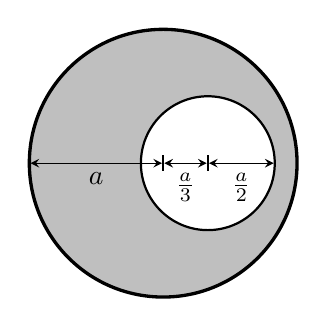
\begin{tikzpicture}[scale=1.7, >=stealth]
    \def\radius{1}
    \filldraw[fill = gray!50, draw=black, very thick] (0, 0) circle (\radius);
    \filldraw[fill=white, draw=black, thick] (\radius/3, 0) circle (\radius/2);
    \draw[|<->|] (0, 0) -- (-\radius, 0) node[midway, below] {$a$};
    \draw[|<->|] (0, 0) -- (\radius/3, 0) node[midway, below] {$\frac{a}{3}$};
    \draw[|<->|] (\radius/3, 0) -- (\radius/3 + \radius/2, 0) node[midway, below] {$\frac{a}{2}$};
  \end{tikzpicture}
  \end{center}
  We see that this situation is not spherically symmetric so we cannot use Gauss's method directly.
  However, we can model the situation as the superposition of a complete sphere of radius $a$ centered at the origin with constant charge density $\rho_0$ and another complete sphere of radius $\frac{1}{2}a$ centered at $\vec{x}_0 = (\frac{1}{3}a, 0, 0)$ with charge density $-\rho_0$.

  We first need to calculate the uniform charge density $\rho_0$ in the charged part of the sphere:
  \[
    \rho_0 = \frac{Q}{\frac{4}{3}\pi a^3 - \frac{4}{3} \pi \left(\frac{1}{2}a\right)^3} = \frac{6Q}{7\pi a^3}
  \]

  We can reuse the result from \cref{chargedBall} to see that when $|\vec{x}| > a$, we have:
  \[
    \phi = \frac{\rho_0 a^3}{3 \varepsilon_0 |\vec{x}|} - \frac{\rho_0 (\frac{1}{2}a)^3}{3 \varepsilon_0 |\vec{x} - \vec{x}_0|} = \frac{2 Q}{7\pi \varepsilon_0}\left[\frac{1}{|\vec{x}|} - \frac{1}{8|\vec{x} - \vec{x}_0|}\right]
  \]
\end{example}
\section{Point Sources}
Consider Poisson's equation $\nabla^2 \phi = f$ in $\R^3$ with a spherically symmetric source term that is non-zero only in the region $|\vec{x}| \leq \varepsilon$ and total source strength $F = \int_{|\vec{x}| \leq \varepsilon} f \d{V}$.

For $R \geq \varepsilon$, we have $F_R = F$, so applying Gauss's flux method from \cref{gaussFluxSpherical}, we find that:
\[
  \phi'(R) = \frac{F}{4 \pi R^2}\ \forall R \geq \varepsilon
\]
Hence by integrating:
\[
  \phi(r) = -\frac{F}{4\pi r} + C\ \forall r \geq \varepsilon
\]
We then choose the constant $C = 0$ so that $\phi(r) \to 0$ as $r \to \infty$ by convention.

Continued next lecture.
\end{document}
